\documentclass{article}

% ------------------------------------ %
%             Document Info            %
% ------------------------------------ %

\usepackage{../../../../LaTeX-Preamables/Clean}
\usepackage[makeroom]{cancel}
\begin{document}

% ------------------------------------ %
%                Header                %
% ------------------------------------ %

\section*{Question 1}

\begin{center}
    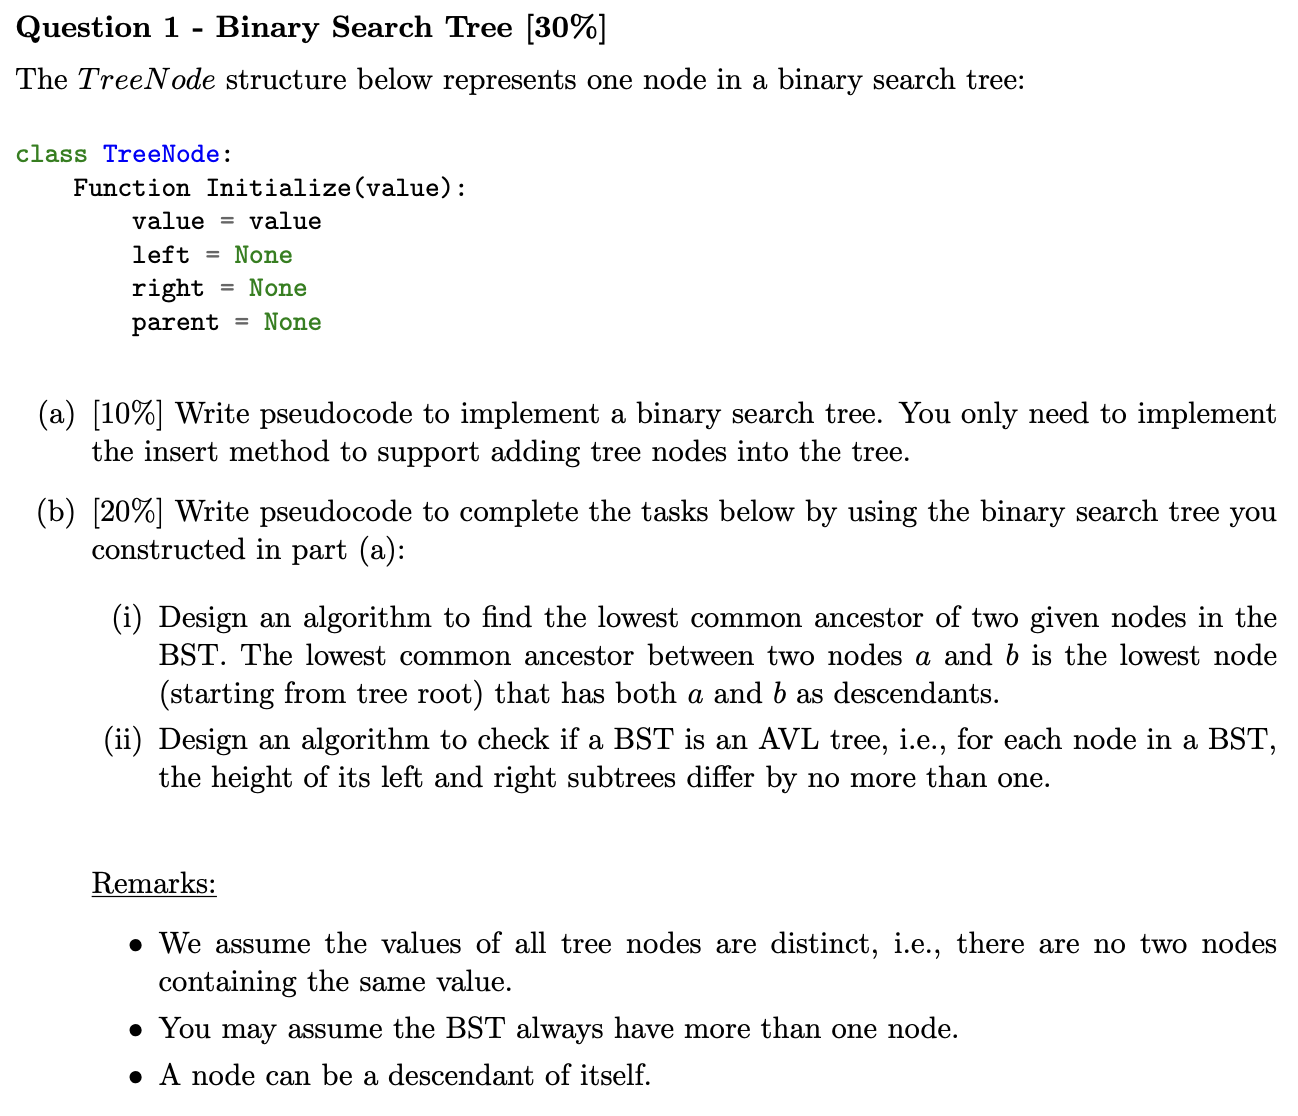
\includegraphics[width=\linewidth]{img/1.png}
\end{center}

\subsection*{Question 1a}
\lstinputlisting[language=Python, basicstyle=\footnotesize\ttfamily, firstline=9, lastline=32]{1.py}

\subsection*{Question 1b}
\lstinputlisting[language=Python, basicstyle=\footnotesize\ttfamily, firstline=35, lastline=53]{1.py}

\section*{Question 2}

\begin{center}
    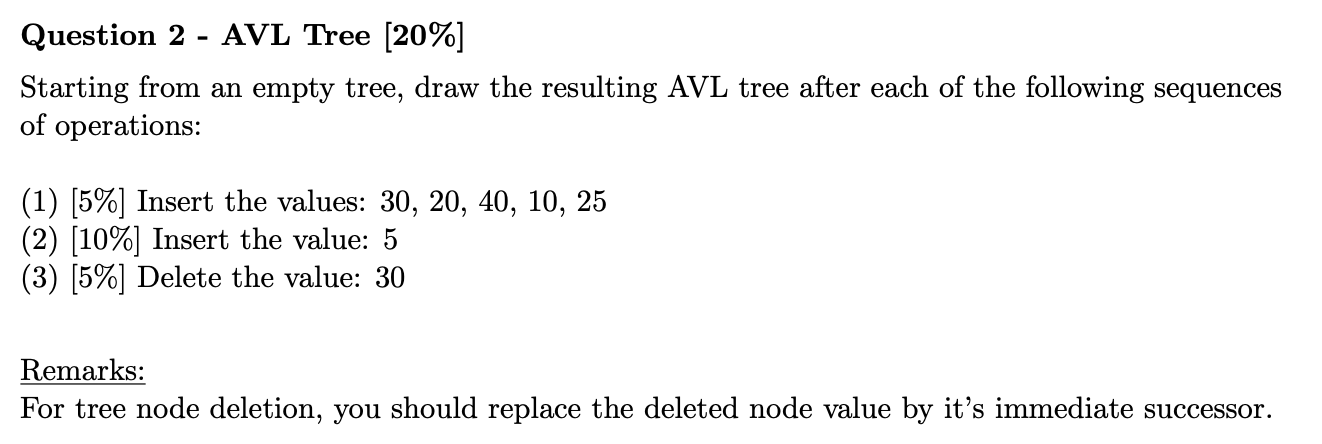
\includegraphics[width=\linewidth]{img/2.png}
\end{center}
\begin{center}
    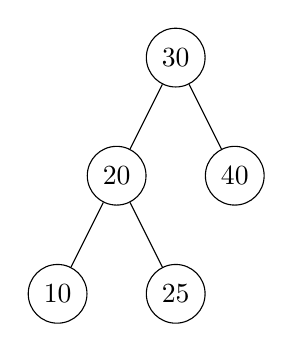
\begin{tikzpicture}
        \begin{scope}[every node/.style={circle,draw}]
            \node {30}
            child {node {20}
                    child {node {10}}
                    child {node {25}}
                }
            child {node {40}};
        \end{scope}
    \end{tikzpicture}
    \hspace{1cm}
    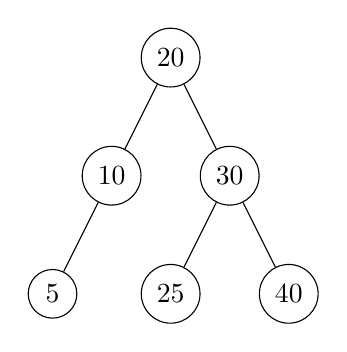
\begin{tikzpicture}
        \begin{scope}[every node/.style={circle,draw}]
            \node {20}
            child {node {10}
                    child {node {5}}
                    child[missing]
                }
            child {node {30}
                    child {node {25}}
                    child {node {40}}
                };
        \end{scope}
    \end{tikzpicture}
    \hspace{1cm}
    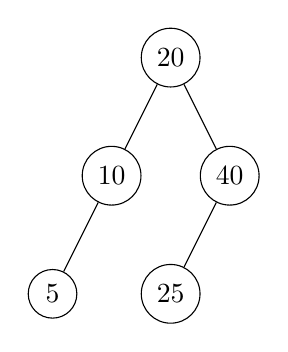
\begin{tikzpicture}
        \begin{scope}[every node/.style={circle,draw}]
            \node {20}
            child {node {10}
                    child {node {5}}
                    child[missing]
                }
            child {node {40}
                    child {node {25}}
                    child[missing]
                };
        \end{scope}
    \end{tikzpicture}
\end{center}

\section*{Question 3a}

\begin{center}
    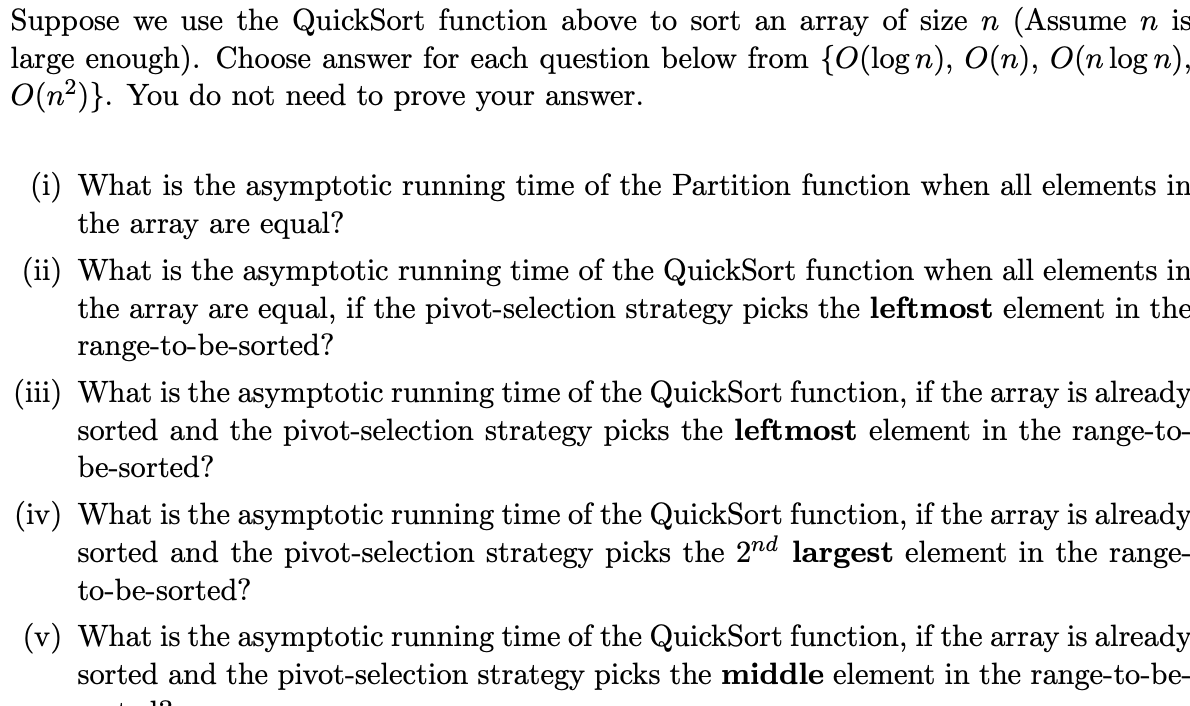
\includegraphics[width=\linewidth]{img/3a.png}
\end{center}

\begin{enumerate}
    \item[(i)] $O(n)$ as the algorithm is linear.
    \item[(ii)] $O(n^2)$ as picked smallest / largest element as pivot.
    \item[(iii)] $O(n^2)$ as picked smallest element as pivot.
    \item[(iv)] $O(n^2)$ as $n-2$ partitions.
    \item[(v)] $O(n \log n)$ as standard.
\end{enumerate}

\section*{Question 3b}

\begin{center}
    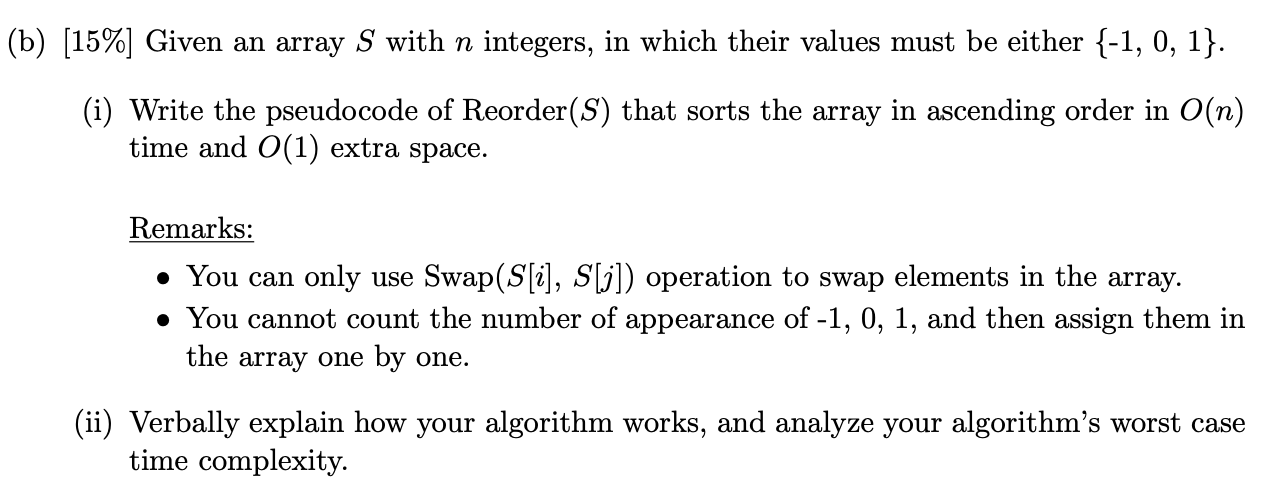
\includegraphics[width=\linewidth]{img/3b.png}
\end{center}

\lstinputlisting[language=Python, basicstyle=\footnotesize\ttfamily, firstline=5, lastline=35]{3b.py}

\section*{Question 4}

\begin{center}
    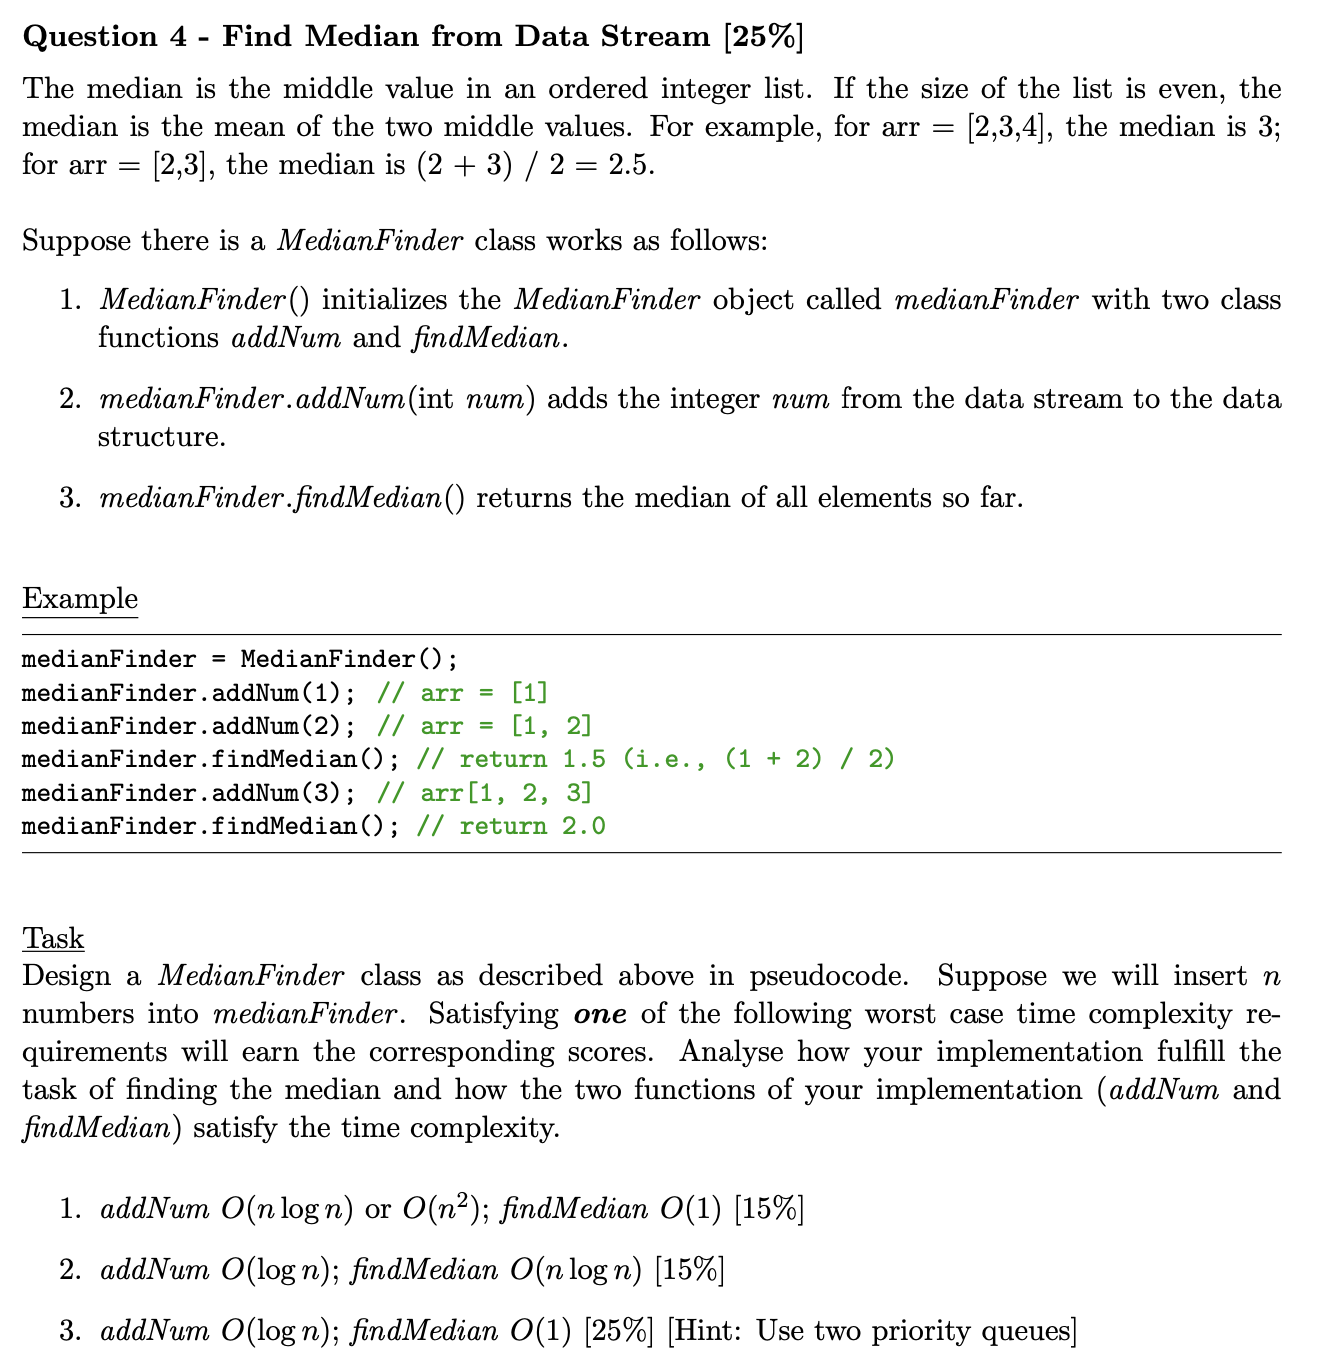
\includegraphics[width=\linewidth]{img/4.png}
\end{center}

\lstinputlisting[language=Python, basicstyle=\footnotesize\ttfamily]{4.pseudocode}

addNum is implemented using two heaps: max-heap and min-heap, which they store the larger and smaller halves of the numbers, and balances the size of the two heaps when adding a number. The queuing and dequeuing of the numbers are done in $O(\log n)$ time complexity, so addNum is $O(\log n)$.

The balancing ensure that the top of min-heap is the median in the case that there are odd number of elements, and if not then the median is the average of the top of the two heaps. The time complexity of finding the median is hence $O(1)$, as we just have to peek the top of the heaps.

\end{document}
